\section{The Backpropagation algorithm}

\definecolor{darkgreen}{rgb}{0,0.6,0}
\definecolor{darkcyan}{rgb}{0,0.5,0.5}
\definecolor{darkyellow}{rgb}{0.5,0.5,0}
\definecolor{mangenta}{rgb}{1,0,1}

\begin{frame}\frametitle{\secname}

The Backpropagation algorithm is a method for computing gradients by using the chain rule efficiently.
\mode<article>{\eqref{eq:gradient_terms} shows us how the gradient breaks down into (1) an error term and (2) a term dependent on the type of model chosen. Specifically:
}	
\begin{equation}
	\textcolor{orange}{	\frac{\partial y(\vec{x}; \vec{w})}{
			\partial {w}_{ij}^{v'v}}}
    \label{eq:model_term}
\end{equation}
\mode<article>{
The Backpropagation algorithm handles the computation of the term in \eqref{eq:model_term} for neural networks such as the one depicted in \figref{fig:example_mlp}.
}
\end{frame}

% -----------------------------------------------------------------------------
\begin{frame} \frametitle{Gradients in neural networks}
    
    \mode<article>{
    The Backpropagation algorithm is not tied to any specific neural architecture. We will therefore attempt to formulate how it works in the general sense.\\
    
    Let $w^{v'v}_{ij}$ be the weight connecting neuron $j$ in layer $v$ to neuron $i$ in layer $v'$, In order to compute $\frac{\partial y(\vec{x}; \vec{w})}{
			\partial {w}_{ij}^{v'v}}$ we need to identify the following:
    \begin{itemize}
        \item $P(v, j)$: the set of immediate parent nodes feeding input into neuron $(v, j)$,
        \item $C(v', i)$: the set of immediate children nodes which neuron $(v', i)$ provides with input
    \end{itemize}
    }
    
    \begin{figure}[h]
    \centering   
    \includegraphics[height=3cm]{img/section1_fig20_mini_multicolor.pdf}
    \mode<article>{
    \caption{Nodes $(v,j)$ and $(v', i)$ are directly connected via the weight $w^{v'v}_{ij}$. The bias node for neuron $(v,j)$ is included in the set of its parent nodes.}
    }
    \label{fig:connection_ij}
    \end{figure}
    
    \mode<article>{
    $h^{v'}_{i}$ measures the total input arriving at neuron $i$ in layer $v'$.
    $h^{v'}_{i}$ is the weighted sum of this neuron's parent activations:
    }
    
    \mode<presentation>{\vspace{-5mm}
    }
    \begin{equation}
            {\color{darkgreen}h_i^{v'}} 
            := 
            \kern-2ex
            \sum_{(\mu,k) \in P(v',\,i)}
            \kern-2ex
            w_{ik}^{v'\mu}\; 
            f_k^\mu\big( {\color{teal} h_k^\mu} \big)   
            \label{eq:total_input_vi},
    \end{equation}
    
    \mode<article>{
    where $\mu$ and $k$ in \eqref{eq:total_input_vi} serve as indices for describing the position of each parent node in $P(v', i)$ in the network.
    }
    \mode<presentation>{\vspace{-5mm}
    }
    
    \pause 
    \question{How does $w_{ij}^{v'v}$ contribute to the error?
    \slidesonly{$\frac{\partial y(\vec{x}; \vec{w})}{\partial w_{ij}^{v'v}} = \ldots$
    \pause
    }}\\
    
    \mode<article>{
    - The contribution is measured by applying the chain rule:
    }
    \mode<presentation>{\vspace{-9mm}
    }
    
    \begin{eqnarray}
        \frac{\partial y(\vec{x}; \vec{w})}{\partial w_{ij}^{v'v}}
            = \underbrace{\frac{\partial y(\vec{x}; \vec{w})}
                {{\color{darkgreen}\partial h_i^{v'}}} }_{ 
                    \substack{\coloneqq\;{\color{red}\delta_i^{v'}} \\
                    \text{``local error''} \\
                    \text{at neuron} \\
                    (v', i)}
                }
              \cdot 
              \underbrace{\frac{{\color{darkgreen}\partial h_i^{v'}}}
                {\partial w_{ij}^{v'v}}}_{
                    \substack{=\;f_j^v({\color{teal} h_j^v}) \\
                    \text{activity} \\
                    \text{of neuron} \\
                    (v, j)}}
                \label{eq:input_output_terms}
    \end{eqnarray}
    
    \mode<article>{
    \eqref{eq:input_output_terms} breaks the contribution of  $w_{ij}^{v'v}$ to the network's output into two parts:
    \begin{enumerate}
     \item The contribution of $h^{v'}_{i}$ to the network's response $y(\vec x; \vec w)$. This is referred to as the ``local error'' at neuron $(v',i)$. The efficiency of the Backpropagation algorithm is based on how it computes the ``local error'' denoted by $\delta_i^{v'}$ for neuron $(v', i)$ and all other neurons in the network.
     \item The contribution of $h^{v'}_{i}$ due to one of its inputs, namely neuron $(v,j)$ which is weighted by $w_{ij}^{v'v}$. We already have everything to compute this term and that is by taking the definition of $h^{v'}_{i}$ in \eqref{eq:total_input_vi} and taking the derivative w.r.t. $w_{ij}^{v'v}$. 
     This should be straightforward since only a single term in the sum depends on $w_{ij}^{v'v}$:
         \begin{equation}
            \frac{{\color{darkgreen}\partial h_i^{v'}}}
            {\partial w_{ij}^{v'v}}
            =  \frac{\partial}
            {\partial w_{ij}^{v'v}}
            \left(
            \sum_{(\mu,k) \in P(v',\,i)}
            \kern-3ex
            w_{ik}^{v'\mu}\; 
            f_k^\mu\big( {\color{teal} h_k^\mu} \big){}
            \right)
            = \underbrace{f_j^v({\color{teal} h_j^v})}_{
            \substack{
                    \text{activity} \\
                    \text{of neuron} \\
                    (v, j)
                    }}
        \end{equation}
    \end{enumerate}
    }
\end{frame}

\begin{frame}\frametitle{The Backpropagation algorithm}
    The Backpropagation algorithm is composed of two stages:
    \begin{enumerate}
     \item \textbf{forward propagation} (forward pass)
     \mode<article>{: Given some input $\vec x$, compute the activities of all neurons and the response of the network.}
     \item \textbf{backward propagation} (backward pass)
     \mode<article>{: Given the response of the network, recursively calculate the local errors starting with the output node and work your way backward through the network.}
    \end{enumerate}
\end{frame}

\subsection{Forward and backward propagation}

% -----------------------------------------------------------------------------
\begin{frame} \frametitle{The Backpropagation algorithm}
    \mode<presentation>{
	\only<1,2>{\placeimage{9.5}{1}{img/section1_fig20_mini_multicolor.pdf}{width=4.8cm}}
	\only<3->{\placeimage{9.5}{1}{img/section1_fig20_mini_back_multicolor.pdf}{width=4.8cm}}
    }
    \mode<presentation>{ \vspace{11mm} }
	\begin{enumerate}
		\item \textbf{forward propagation}: calculate activities 
				$f_i^{v'}({\color{darkgreen}h_i^{v'}})$
				{\small(parents $\rightarrow$ children)}
				$$	
					{
					%\color{darkgreen}
					h_j^0
					} 
						\;:=\; \mathrm{x}_j \,, 
					\quad 
					{\color{darkgreen}h_i^{v'}}
		   			\,= \kern-2ex\smallsum{(\mu,k) \in P(v',\,i)}{} \kern-2ex
	   			w_{ik}^{v'\mu}\;  f_k^\mu\big( {\color{teal} h_k^\mu} \big) \,,
					\quad
					y(\vec{x}; \vec{w})\,=\, f_1^L({\color{blue}h_1^L})
				$$\\\vspace{-2mm}
	\only<1>{	
		\mode<presentation>{
		\begin{center}
		\vspace{2mm}
		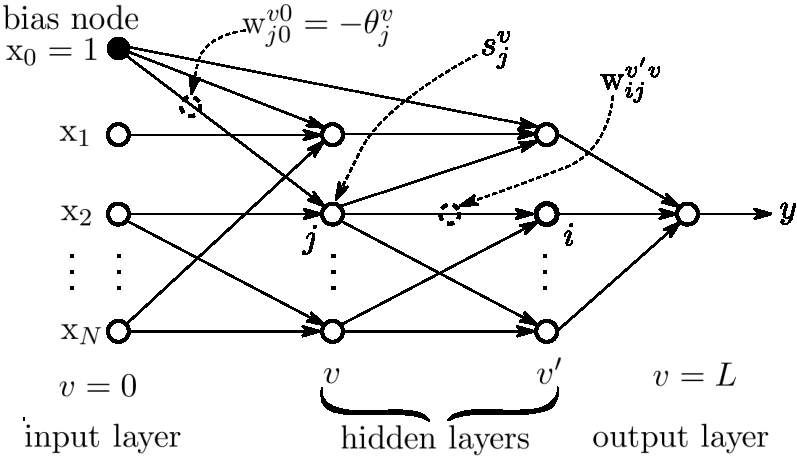
\includegraphics[height=4cm]{img/section1_fig14}
		\end{center}
		}
	}
	\only<2>{	
		\mode<presentation>{
		\begin{center}
		\vspace{2mm}
		\includegraphics[height=4cm]{img/section1_fig14_fwd}
		\end{center}
		}
	}
	\only<3->{
		\item \textbf{backpropagation}: calculate ``local errors'' 
				$\color{red}\delta_i^{v'}$
				{\small(children $\rightarrow$ parents)}
				\vspace{-1mm}
				%~ \begin{eqnarray*} 
				%~ \end{eqnarray*}
				\begin{eqnarray} 
				{\color{red} \delta_1^L}
				&=& \frac{\partial y(\vec{x}; \vec{w})} {{\color{blue}\partial h_1^{L}}}
					= [f_1^{L}]'({\color{blue} h_1^{L}})
							%\;\;\text{for}\;v'=L
							\\
					{\color{red}\delta_i^{v'}} 
					\only<3>{
						&=&  \frac{\partial y(\vec x; \vec w)}{\color{darkgreen}\partial h^{v'}_{i}}
						\qquad \text{``local error'' at neuron }(v', i)
                        \label{eq:delta_step1}\\
						}
					\only<4->{
						&=&  \kern-3ex\sum\limits_{(v''\hspace{-1mm},\,k) \in C(v',\,i)}{
						\underbrace{
							\smallfrac{\partial y(\vec{x}; \vec{w})}
								{{\color{blue}\partial  h_k^{v''}}}
							}_{{\color{red}\delta_k^{v''}}} 
						\;\kern1.5ex\cdot \kern-2.5ex\;
						\underbrace{\smallfrac
								{{\color{blue}\partial h_k^{v''}} }
								{{\color{darkgreen}\partial h_i^{v'}}}
							}_{{w}_{ki}^{v''v'} \kern-.5ex\cdot\kern.5ex
								[f_i^{v'}]'({\color{darkgreen}h_i^{v'}}) }}
                            \label{eq:delta_step2}
                                \notesonly{\\&=&  \kern-3ex\sum\limits_{(v''\hspace{-1mm},\,k) \in C(v',\,i)}{
						{\kern-2ex {\color{red}\delta_k^{v''}}}
                        \cdot\,
						{{w}_{ki}^{v''v'} \kern-.5ex\kern.5ex
								[f_i^{v'}]'({\color{darkgreen}h_i^{v'}}) }}}
                                \notesonly{\\ \kern-3ex&=&\;\;\; }%\,,
                                \slidesonly{\kern-3ex=\;\;\; }%\underbrace{
							[f_i^{v'}]'({\color{darkgreen}h_i^{v'}}) 
							\kern-3ex\sum_{(v''\hspace{-1mm},\,k) \in C(v',\,i)}\kern-3ex
							{\color{red}\delta_k^{v''}} 
							{w}_{ki}^{v'' v'} 
						}
						%}_{{\color{red} \delta_i^L}\;=\;
						%	[f_i^{L}]'({\color{darkgreen} h_i^{L}})
						%	\;\;\text{for}\;v'=L}
				\end{eqnarray}
		}
		\only<5->{
		\vspace{-1mm}
		\item[] \textbf {weight update}: using activities and local errors
        \begin{equation}
				{w}_{ij}^{v'v}
				\; \leftarrow \; 
				{w}_{ij}^{v'v} - \eta \cdot
				\smallfrac{\partial e}{\partial{w}_{ij}^{v'v}}
				\;=\; {w}_{ij}^{v'v} - \eta \, \cdot 
				\smallfrac{\partial e}{\partial y(\vec{x}; \vec{w})} \cdot
				\only<5>{
				\smallfrac{\partial y(\vec{x}; \vec{w})}{\partial{w}_{ij}^{v'v}}\hspace{8.5mm}
				}
                \slidesonly{
				\only<6>{
				{\color{red} \delta_i^{v'}} \kern-.5ex\cdot
			   			f_j^v( {\color{teal}h_j^v} )
			   	}}
        \end{equation}
        \notesonly{
        \begin{equation}
				{w}_{ij}^{v'v}
				\quad \leftarrow \quad 
                {w}_{ij}^{v'v} - \eta \, \cdot
				\smallfrac{\partial e}{\partial y(\vec{x}; \vec{w})} \cdot
				{
				{\color{red} \delta_i^{v'}} \kern-.5ex\cdot
			   			f_j^v( {\color{teal}h_j^v} )
			   	}
        \end{equation}
        }
			}
	\end{enumerate}
	%{\scriptsize
	%Computational complexity: $O(n)$, $n$: number of weights \& thresholds}
    
\end{frame}

\mode<article>{
    To understand how the ``local error'' at neuron $(v',i)$ goes from its definition in \eqref{eq:delta_step1} to \eqref{eq:delta_step2}, one needs to look at the propagation from $(v',i)$ forwards to all its immediate children nodes in $C(v', i)$. Let $(v'', k)$ describe a neuron positioned deeper in the network and connected to $(v',i)$, making it one of its children and, in turn, making $(v',i)$ one of the parents of $(v'', k)$.\\
    Analogous to how we compute in ${\color{darkgreen}h_i^{v'}}$ in \eqref{eq:total_input_vi}:
    
    \begin{align}
            {\color{blue}h_k^{v''}} 
            :=& 
            \kern-2ex
            \sum_{(\mu,\,l) \in P(v'',\,k)}
            \kern-2ex
            w_{kl}^{v''\mu}\; 
            f_l^\mu\big( {h_l^\mu} \big)   
            \label{eq:total_input_vddk}\\
            =&\; \ldots \,+\,{}
            w_{ki}^{v''v'}\; 
            f_i^{v'}\big( {\color{darkgreen}h_i^{v'}})
            \,+\, \ldots
    \end{align}
    
    Since only one term in this sum depends on ${\color{darkgreen} h_i^{v'}}$:
    \begin{align}
    \frac{{\color{blue}\partial h_k^{v''}} }{{\color{darkgreen}\partial h_i^{v'}}}
    \;&= \;
    \frac{\partial}{\color{darkgreen}\partial h_i^{v'}}
    \left(
    w_{ki}^{v''v'}\; 
            f_i^{v'}\big( {\color{darkgreen}h_i^{v'}})
    \right)\\
    \;&= \; w_{ki}^{v''v'} \,
    \frac{\partial}{\color{darkgreen}\partial h_i^{v'}}
            f_i^{v'}\big( {\color{darkgreen}h_i^{v'}})\\
    \;&= \; {{w}_{ki}^{v''v'} \;
    [f_i^{v'}]'({\color{darkgreen}h_i^{v'}}) }
    \end{align}
}

\clearpage

\subsection{Example: MLP with fully connected layers}

\mode<article>{
We will apply the Backpropagation algorithm to an MLP as depicted by \figref{fig:mlp_fc}. All neurons in one layer are connected with all nodes of the next layer. The layers are therefore \emph{fully connected}. This implies that the weights between consecutive layers make up a \emph{dense} weight matrix. This allows us to express the formulas using vector notation.  
}

\begin{frame}\frametitle{\subsecname}
    \begin{figure}[h]
    \centering   
    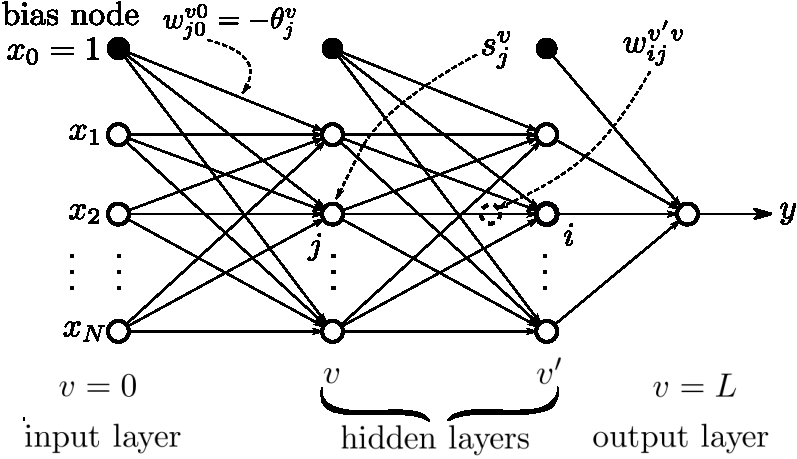
\includegraphics[height=5cm]{img/section1_fig14_fc}
    \mode<article>{
    \caption{MLP with fully connected layers}
    }
    \label{fig:mlp_fc}
    \end{figure}
    
\notesonly{Recall that the purpose of the Backpropagation algorithm is to compute the gradients. Therefore, the task is to obtain an expression for computing }\slidesonly{compute} the gradients for all weights and biases in this network:\\

\pause

\question{What is the procedure for the Backpropagation algorithm?}\\

\mode<article>{
- The procedure is:
\begin{enumerate}
 \item forward pass: compute ${h^{v}_{i}}$ for $v = 0,\ldots,L$,\\
 \item backward pass: backpropagation of ``local errors'' (i.e. compute ${\color{red}\delta^{v}_{i}}$).
\end{enumerate}
}
\end{frame}

\subsubsection{The forward pass}
\begin{frame}\frametitle{\subsubsecname}
    
    \mode<presentation>{
    \placeimage{7.4}{1}{img/section1_fig14_fc_nolayers}{width=6.7cm}
    \begin{textblock}{4}(0.5,2)
    \begin{equation}
    \boxed{
        {\color{darkgreen}h_i^{v'}}
        \,= \kern-2ex
        \smallsum{(\mu,k) \in P(v',\,i)}{}
        \kern-2ex
        w_{ik}^{v'\mu}\; f_k^\mu\big( {\color{teal} h_k^\mu} \big)
    }
    \end{equation}
    \end{textblock}
    \vspace{1cm}
    }
    
    Compute ${h^{v}_{i}}$ \only<1>{for $v = 0,\ldots,L$}:

    \begin{itemize}
    \only<1,2>{
        \item $v=0$ (input layer):\\ \slidesonly{\vspace{-3mm}}
        \begin{flalign}
            h^{0}_{j} &=
            \slidesonly{\only<1>{&&}}
            \only<2>{
                              x_{j}\;,   & j=1,\ldots,N&&\\
                h^{0}_{0}  &=  x_{0} = 1          & (\text{bias node})\\
                \vec h^{0} &= \vec x     & (\text{bias included})\\
                f^0_{j}(h) :\kern-0.5ex&= h & \text{ (identity function)}\\
                %\Rightarrow\; 
                \vec f^0(\vec h) &= \vec x & \text{ (identity, bias included)}
            }
        \end{flalign}
    }
    \only<3,4>{
        \slidesonly{\vspace{5mm}}
        \item $v=1$ (1\textsuperscript{st} hidden layer with $N_{1} \text{ nodes}$):\\ \slidesonly{\vspace{-2mm}}
        \begin{flalign}
        h^{1}_{j} &= 
        \slidesonly{\only<3>{&&}}
        \only<4>{
            \smallsum{k=0}{N} w_{jk}^{10}\;  f_k^0\big( {h_k^0} \big) = {\vec w_{j}^{10}}^{\top} \vec h^0 & (\text{bias included})&&\\
            \vec h^{1} &= {\vec W^{10}}^{\top} \vec h^0 = {\vec W^{10}}^{\top} \vec x &(\text{biases included})\\
            f^1_{j}(h) :\kern-0.5ex&= \text{e.g. }\tanh(h),  &j=1,\ldots,N_{1}\\ f^1_{0}(h) :\kern-0.5ex&= h &\text{(identity for bias)}\\
        }
        \end{flalign}
    }
    \only<5,6>{
        \item $v=2$ (2\textsuperscript{nd} hidden layer with $N_{2} \text{ nodes}$):\\ \slidesonly{\vspace{-7mm}}
    % temporarily change footnote marks to symbols so not to confuse with exponents
    %\renewcommand*{\thefootnote}{\fnsymbol{footnote}}
        \begin{flalign}
        h^{2}_{i} &=
        \slidesonly{\only<5>{&&}}
        \only<6>{
            \smallsum{j=0}{N_{1}} w_{ij}^{21}\;  f_j^1\big( {h_j^1} \big) = 
            {\vec w_{i}^{21}}^{\top} 
            %\overbrace{
            \vec f^{1}(\vec h^1)
            %}^{
            %\vec s^1
            %} 
            &(\text{bias included})&&\\
            \vec h^{2} &= {\vec W^{21}}^{\top} \vec f^{1}(\vec h^1) &(\text{biases included})\\
            f^2_{i}(h) :\kern-0.5ex&= \text{e.g. }\tanh(h) &i=\mathbf{1},\ldots,N_{2}\\
            f^2_{0}(h) :\kern-0.5ex&= h &\text{(identity for bias)}\\
        }
        \end{flalign}
        }
    \only<7,8>{
        \item $v=L$ (output layer):\\ \slidesonly{\vspace{-4mm}}
        \begin{flalign}
        h^{L}_{1} &=
        \slidesonly{\only<7>{&&}}
        \only<8>{
            \smallsum{i=0}{N_{2}} w_{1i}^{L2}\;  f_i^1\big( {h_i^1} \big) = {\vec w_{1}^{21}}^{\top} \vec f^{2}(\vec h^2) &(\text{bias included})&&\\
            y(\vec x; \vec w) &= f^L_{1}(h^{L}_{1})&&\\
            f^L_{1}(h) :\kern-0.5ex&= \text{e.g. logistic function (sigmoid)}\\
        }
        \end{flalign}
    }
    \end{itemize}
    
\end{frame}

\subsubsection{The backward pass}

\begin{frame}\frametitle{\subsubsecname}
    \mode<presentation>{
    \placeimage{7.4}{1}{img/section1_fig14_fc_nolayers}{width=6.7cm}
    \begin{textblock}{4}(0.5,2)
    \begin{equation}
    \boxed{
        {\color{red}\delta_i^{v'}}
        =
        [f_i^{v'}]'({\color{darkgreen}h_i^{v'}}) 
        \kern-3ex\sum_{(v''\hspace{-1mm},\,k) \in C(v',\,i)}\kern-3ex
        {\color{red}\delta_k^{v''}} 
        {w}_{ki}^{v'' v'}
            }
    \end{equation}
    \end{textblock}
    \vspace{2cm}
    }
    
    Compute ${\color{red}\delta^{v}_{i}}$:
    
    % temporarily change footnote marks to symbols so not to confuse with exponents
    \renewcommand*{\thefootnote}{\fnsymbol{footnote}}
    \begin{itemize}
    \only<1,2>{
        \item $v=L$ (output layer):\\ \slidesonly{\vspace{-4mm}}
        \begin{flalign}
            y(\vec x; \vec w) &= f^L_{1}(h^{L}_{1})&&\\
            f^L_{1}(h) &= \text{e.g. logistic function (sigmoid)}\\
            {\color{red}\delta^{L}_{1}}  &= \frac{\partial y(\vec{x}; \vec{w})} {{\color{blue}\partial h_1^{L}}} =
        \only<2>{
                [f_1^{L}]'({\color{blue} h_1^{L}})
        }
        \end{flalign}
    }

    \only<3,4>{
        \item $v=2$ (2\textsuperscript{nd} hidden layer with $N_{2} \text{ nodes}$):\\ \slidesonly{\vspace{-7mm}}
        \begin{flalign}
            f^2_{i}(h) :\kern-0.5ex&= \text{e.g. }\tanh(h), &i=1,\ldots,N_{2}&&\\
            f^2_{0}(h) :\kern-0.5ex&= h &\text{(identity for bias)}\\
            {\color{red}\delta^{2}_{i}} &=
        \only<4>{
                [f_i^{2}]'({\color{darkgreen}h_i^{2}})\;
                {\color{red}\delta_1^{L}} \,
                {w}_{1i}^{L2}
                &(\text{bias }{\scriptsize{w}_{0i}^{L2}}\text{ excl.})\\
             {\color{red} \vec \delta^{2}} &=\; [\vec f^{2}]'({\color{darkgreen}\widetilde{\vec h}^{2}}) \odot ({\color{red}\delta_1^{L}} \cdot {\widetilde{\vec w}_{1}^{L2}})
        \notesonly{ \footnotemark }
        %\notesonly{ \footnotemark }
        }
        \end{flalign}
        \notesonly{
            \footnotetext{
            $\widetilde{\vec {w}}_{1}^{L2} \; \corresponds \; {\vec {w}}_{1}^{L2}$ without the bias node.\\
            ${\color{darkgreen} {\vec{\widetilde{h}}^{2}}}  \; \corresponds \; {\color{darkgreen} {\vec{{h}}^{2}}}$ without the bias node.
            ``$\odot$'' stands for elementwise multiplication, while ``$\cdot$'' stands for the dot product.
            }
        }
        %\notesonly{
        %\footnotetext{``$\odot$'' stands for elementwise multiplication, while ``$\cdot$'' stands for the dot product.}
        %}
        }
    \only<5,6>{
        \item $v=1$ (1\textsuperscript{st} hidden layer with $N_{1} \text{ nodes}$):\\ \slidesonly{\vspace{-5mm}}
        \begin{flalign}
            f^1_{j}(h) :\kern-0.5ex&= \text{e.g. }\tanh(h),  &j=1,\ldots,N_{1}\\ f^1_{0}(h) :\kern-0.5ex&= h &\text{(identity for bias)}&&\\
            {\color{red}\delta^{1}_{j}}
             &=
        \only<6>{
                [f_j^{1}]'({\color{darkgreen}h_j^{1}}) 
                \kern-.5ex\sum_{k=1}^{N_{2}}\kern-.5ex
                {\color{red}\delta_k^{2}} \,
                {w}_{{\color{magenta}kj}}^{21} %\\%&
                %\notesonly{\\&}
                %= 
                %[f_j^{1}]'({\color{darkgreen}h_j^{1}})\,
                %{\color{red} {\vec{\widetilde{\delta}}^{2}}^{\top}}
                %\widetilde{\vec {w}}_{j}^{21}
                &(\text{bias k=0  excl.})\\%TODO: vector notation for this
                %\notesonly{\\[3mm]}\slidesonly{\\}
                %(\text{skip }k=0)\\
                %}
        %\end{flalign}
        %\vspace{-2mm}
        %\begin{flalign}
        %\only<6>{
            {\color{red} \vec \delta^{1}}
             &=
                [\vec f^{1}]'({\color{darkgreen}\widetilde{\vec h}^{1}})
                \odot
                (
                \kern-.5ex\cdot
                \widetilde{\vec {W}}^{21}
                {\color{red} {\vec \delta^{2}}}) \notesonly{ \footnotemark }
                & \\
             %&= 
                %[\vec f^{1}]'({\color{darkgreen}h^{1}})
                %\odot
                %({{\vec {\widetilde{W}}}^{21}}^{\top} 
                %\kern-.7ex\cdot
                %{\color{red} {\vec{\widetilde{\delta}}^{2}}^{\top}})
                %& (\vec A\, \vec B)^{\kern-.5ex\top}\kern-1ex=\vec B^{\top}\kern-.8ex\vec A^{\kern-.5ex\top}
        }
        \end{flalign}
        \notesonly{
            \footnotetext{
            $\widetilde{\vec {W}}^{21} \; \corresponds \; {\vec {W}}^{21}$ without the bias in each column vector ${\vec {w}}_{j}^{21}$. $w_{\color{magenta}{kj}}^{21}$ refers to row ${\color{magenta}j}$, col. ${\color{magenta}k}$ of $\widetilde{\vec {W}}^{21}$.
            ${\color{darkgreen} {\vec{\widetilde{h}}^{1}}}  \; \corresponds \; {\color{darkgreen} {\vec{{h}}^{1}}}$ without the bias node.
            %${\color{red} {\vec{\widetilde{\delta}}^{2}}^{\top}}  \; \corresponds \; {\color{red} {\vec{{\delta}}^{2}}^{\top}}$ without the bias node (k=0), i.e. ${\color{red} {\vec{\widetilde{\delta}}^{2}}^{\top}}$ is ${\color{red} {\vec{{\delta}}^{2}}^{\top}}$ without ${\color{red} \delta^{2}_{0}}$.
            }
        }
    }
    \only<7,8>{
        \item $v=0$ (input layer):\\ \slidesonly{\vspace{-3mm}}
        \begin{flalign}
                f^0_{j}(h) :\kern-0.5ex&= h & \text{ (identity function)}&&\\
                \vec f^0(\vec h) :\kern-0.5ex&= \vec x &\text{ (bias included)}
                \\
            {\color{red}\delta^{0}_{j}}
             &\;
            \only<8>{
            &
             (\text{Not applicable to observed input})
             }
        \end{flalign}
        \slidesonly{
        \vspace{5mm}
        \begin{equation}
		\boxed{
				{w}_{ij}^{v'v}
				\, \leftarrow \, 
				{w}_{ij}^{v'v} - \eta \cdot
				\smallfrac{\partial e}{\partial y(\vec{x}; \vec{w})} \cdot
				\smallfrac{\partial y(\vec{x}; \vec{w})}{\partial{w}_{ij}^{v'v}}
				\;=\; {w}_{ij}^{v'v} - \eta \cdot
				\smallfrac{\partial e}{\partial y(\vec{x}; \vec{w})} \cdot
				{\color{red} \delta_i^{v'}} \kern-.5ex\cdot
			   			f_j^v( {\color{darkgreen}h_j^v} )
		}
        \end{equation}
        }
    }
    \end{itemize}
    % change footnote marks back to original scheme (numbers)
    \renewcommand*{\thefootnote}{\arabic{footnote}}
    
\end{frame}

\begin{frame}

{\renewcommand{\arraystretch}{1.5} %<- control vertical spacing
\begin{table}[!h]
\centering
\caption{Overview of dimensions}
%\resizebox{\textwidth}{!}
{%
\label{tab:summary_bp} 
\begin{tabular}{|c||c|c|c|}
\hline
\multicolumn{1}{|c||}{layer} & \multicolumn{1}{c|}{parameters}                  & \multicolumn{1}{c|}{total input} & \multicolumn{1}{c|}{``local'' errors}\\ 
\hline \hline
$v=0$
& N/A 
&
\begin{tabular}[c]{@{}l@{}}
    $\vec h^{0} := \vec x$\\
    $\vec h^{0} \in \R^{N+1}$\vspace{2mm}
\end{tabular} 
& N/A\\ 
\hline
$v=1$ 
& \begin{tabular}[c]{@{}l@{}}
    $\vec w_{j}^{10}  \in \R^{N+1}$\\
    $\vec {W}^{10} \in \R^{(N+1) \times N_{1}}$\vspace{2mm}
\end{tabular} 
& \begin{tabular}[c]{@{}l@{}}
    %$\vec h^{1} := \vec f({\vec {W}^{10}}^{\top}\vec x)$\\
    $\vec h^{1} \in \R^{N_{1}+1}$\\
    $\widetilde{\vec h}^{1} \in \R^{N_{1}}$\vspace{2mm}
\end{tabular} 
& \begin{tabular}[c]{@{}l@{}}
    ${\color{red} \vec{\delta}^{1}} \in \R^{N_{1}}$\vspace{2mm}
\end{tabular} \\ 
\hline
$v=2$ 
& \begin{tabular}[c]{@{}l@{}}
    $\vec w_{i}^{21}  \in \R^{N_{1}+1} $\\
    $\vec {W}^{21}  \in \R^{(N_{1}+1) \times N_{2}}$\\
    $\widetilde{\vec {W}}^{21}  \in \R^{(N_{1}) \times N_{2}}$\vspace{2mm}
\end{tabular} 
& \begin{tabular}[c]{@{}l@{}}
    $\vec h^{2} \in \R^{N_{2}+1}$\\
    $\widetilde{\vec h}^{2} \in \R^{N_{2}}$\vspace{2mm}
\end{tabular}
& \begin{tabular}[c]{@{}l@{}}
    ${\color{red} \vec{\delta}^{2}} \in \R^{N_{2}}$ \\
    %${\color{red} \widetilde{\vec{\delta}}^{2}} \in \R^{N_{2}}$\vspace{2mm}
\end{tabular} \\ 
\hline
$v=L$ 
& \begin{tabular}[c]{@{}l@{}}
    $\vec w_{1}^{L2}  \in \R^{N_{2}+1}$\vspace{2mm}
\end{tabular} 
& $h_1^{L} \in \R$ 
& ${\color{red}\delta^{L}_{1}} \in \R$\\ 
\hline
\end{tabular}
}
\end{table}
} % arraystretch
    
\end{frame}

\clearpage

% -----------------------------------------------------------------------------
\definecolor{forward}{rgb}{0,0.7,0}
\definecolor{backward}{rgb}{0.8,0,0}

\subsection{Summary of the Backpropagation for gradient descent}

\begin{frame} \frametitle{\subsecname}
    \mode<presentation>{
	\only<1>{
		\placeimage{10.75}{5.5}{img/MLP_forward.pdf}{width=3.75cm}
		\placeimage{10.75}{8.7}{img/MLP_backward.pdf}{width=3.75cm}
	}}
	
	%\begin{algorithm}[H] 
		%\scriptsize
		\footnotesize
		\DontPrintSemicolon
		initialization of weights and thresholds \\
        
		\While{stopping criterion not met}{
			$\text{gradient}_{ij}^{v'v} := 0 
					\,, \quad \forall w_{ij}^{v'v}$ \\
                    
			\For{$\alpha \in \{1,\ldots,p\}$}{
				${\color{forward}h_i^0} 
					:= x_i^{(\alpha)} \,, \quad \forall i$ 
				\qquad\qquad // {\color{forward}forward propagation}\\
                
				\For{$v' \in \{1,\ldots,L\}$}{
					%~ ${\color{forward} h_i^{v'}} 
						%~ := \sum\limits_{\scriptscriptstyle
							%~ (v',i) \in C(v,j)} w_{ij}^{v'v} 
							${\color{forward}h_i^{v'}}
		   			\;\;=\;\; \kern-2ex\smallsum{(\mu,k) \in P(v',i)}{} \kern-2ex
	   			w_{ik}^{v'\mu}\;  \underbrace{f_k^\mu\big( {\color{forward} h_k^\mu} \big) 
								%~ \underbrace{f_j^v({\color{forward} h_j^{v}})
								}_{\kern-2exx_k^{(\alpha)} \;\text{if}\; 
									v'=1\kern-2ex } \,,
							\quad \forall i$
					\vspace{-1.5mm}
				}
				${\color{backward} \delta_1^L} 
					:= [f_1^L]'({\color{forward}h_1^L}) $%\,, \quad \forall i$ 
				\qquad // {\color{backward}backward propagation}\\
                
				\For{$v' \in \{L-1,\ldots,1\}$} {
					${\color{backward}\delta_i^{v'}} 
						:= [f_{i}^{v'}]'({\color{forward}h_i^{v'}}) 
						\kern-1ex\sum\limits_{(\mu,k) \in C(v',i)}\kern-1ex
						{\color{backward} \delta_k^{\mu}} 
						\, w_{ki}^{\mu v'} \;,
						\quad \forall i$
					\vspace{-2.5mm}
				}
				$\text{gradient}_{ij}^{v'v} := \text{gradient}_{ij}^{v'v}
						+ \frac{\partial e^{(\alpha)}}{\partial y(\vec x; \vec w)}
						 \, {\color{backward}\delta_i^{v'}} 
						 \, f_j^v({\color{forward}h_j^v})
						 \,, \quad \forall w_{ij}^{v'v}$
				\hspace{11mm} // sum
			}
			\notesonly{ // gradient descent step:\\
            
            }
			$\text{gradient}_{ij}^{v'v} := \frac{1}{p} \text{gradient}_{ij}^{v'v}$\\
			% $w_{ij}^{v'v} := w_{ij}^{v'v} - \frac{\hat \eta}{p}
			 $w_{ij}^{v'v} := w_{ij}^{v'v} - \eta
					\, \text{gradient}_{ij}^{v'v} 
					\,, \quad \forall w_{ij}^{v'v}	$
			\slidesonly{\hspace{15mm} // gradient descent step}
					\vspace{-1.5mm}
		}
		%\caption{Backpropagation in feedforward networks}
	%\end{algorithm}
\end{frame}

\subsubsection{Complexity}

\begin{frame}\frametitle{\subsubsecname}

The computational and 
memory complexity of the Backpropagation algorithm is
$\mathcal{O}(n)$, %\quad,{}
where $n$ is the total number of the weights in the network. 
\mode<article>{It is therefore, 
\emph{linear} in the 
number of weights.}

An alternative\slidesonly{:}\notesonly{and very simple method for computing the gradients would be to use }
\pause
\emph{finite differences}.

Let $\widetilde{\vec w}$ denote all parameters of the network except for a single weight $w^{v'v}_{ij}$

\mode<article>{
The idea is to add (subtract) a small offset $\varepsilon$ to (from) $w^{v'v}_{ij}$ in the network, while keeping all other weights $\widetilde{\vec w}$ fixed and measure the change in the error function. Specifically,
}
\begin{equation}
e\big(y_T, y\big(\vec x; \widetilde{\vec w}, {w}^{v'v}_{ij} \pm \varepsilon\big)\big) =: e\big(\widetilde{\vec w}, {w}^{v'v}_{ij} \pm \varepsilon\big) \text{ for brevity}
\end{equation}
\pause
For $\varepsilon \ll 1$ follows:

\begin{equation}
\frac{\partial e\left(y_T, y\left(\vec x; {\vec w}\right)\right)}{\partial {w}^{v'v}_{ij}} =
\frac{
e\big(\widetilde{\vec w}, {w}^{v'v}_{ij} + \varepsilon\big)
+
e\big(\widetilde{\vec w}, {w}^{v'v}_{ij} - \varepsilon\big)
}
{2 \,\varepsilon}
+ \mathcal{O}(\varepsilon^{2})
\label{eq:finitediff}
\end{equation}

\notesonly{
The complexity of the forward propagation remains $\mathcal{O}(n)$. Performed it twice in \eqref{eq:finitediff} is manageable as $\mathcal{O}(2n) \leadsto \mathcal{O}(n)$.
However, this is the complexity for a single weight. Performing this for all $n$ weights in the network increases the complexity of finite differences to $\mathcal{O}(n^{2})$.

However, numerical differentiation such as finite differences remains a useful tool for debugging your Backpropagation algorithm and performing gradient checks.
}

\pause

\slidesonly{
Complexity of finite differences increases to.$\mathcal{O}(n^{2})$. But still good for gradient checks.
}


    
\end{frame}
